\section{Building an Adding Machine}
All of these little units, experiments, and instruction have been moving towards a goal -- to make a primitive electronic calculator. Here, we will be able to add two four-bit numbers using only full adders, toggle switches, and LED blocks, all wired together on a breadboard. At the end of this unit, you will be able to enter two numbers in binary using toggle switches, and read the result on an LED readout, also in binary. There's no reason you have to stop at 4 bits -- the 8-LED block means you could add two 7-bit numbers if you have seven full adders and more toggle switches, without \emph{overflowing} the capabilities of the setup. ``Overflow'' means that you have tried to put numbers into the system that cannot be represented by the computer because they are too large, or else the result is too large to display. 

\subsection*{Wiring up the adders}

Put two sets of toggle switches on a breadboard and, if desired, two 8-LED readouts (one for each set of toggles). Wire up power and ground to the switches and LEDs, and wire the switch outputs to the LED inputs, moving from right to left, because the rightmost digit is the smallest number value in our example, either 0 or 1.

Run wires out from the switches, perhaps using one color for one bank of switches, and a different color for the second bank, to each input of each full adder, and wire up each ``carry-out'' to the next (leftward!) ``carry-in''. The left-most carry-out digit should run to another LED, perhaps not on the 8-LED output, to indicate an overflow. The overflow, a type of error, means the answer is not correctly displayed on the LED output bar.

Run each adder ``sum" wire to each output LED input. In doing this you will have wired up each column of output, meaning you can read off the sum of the two numbers.


\begin{figure}
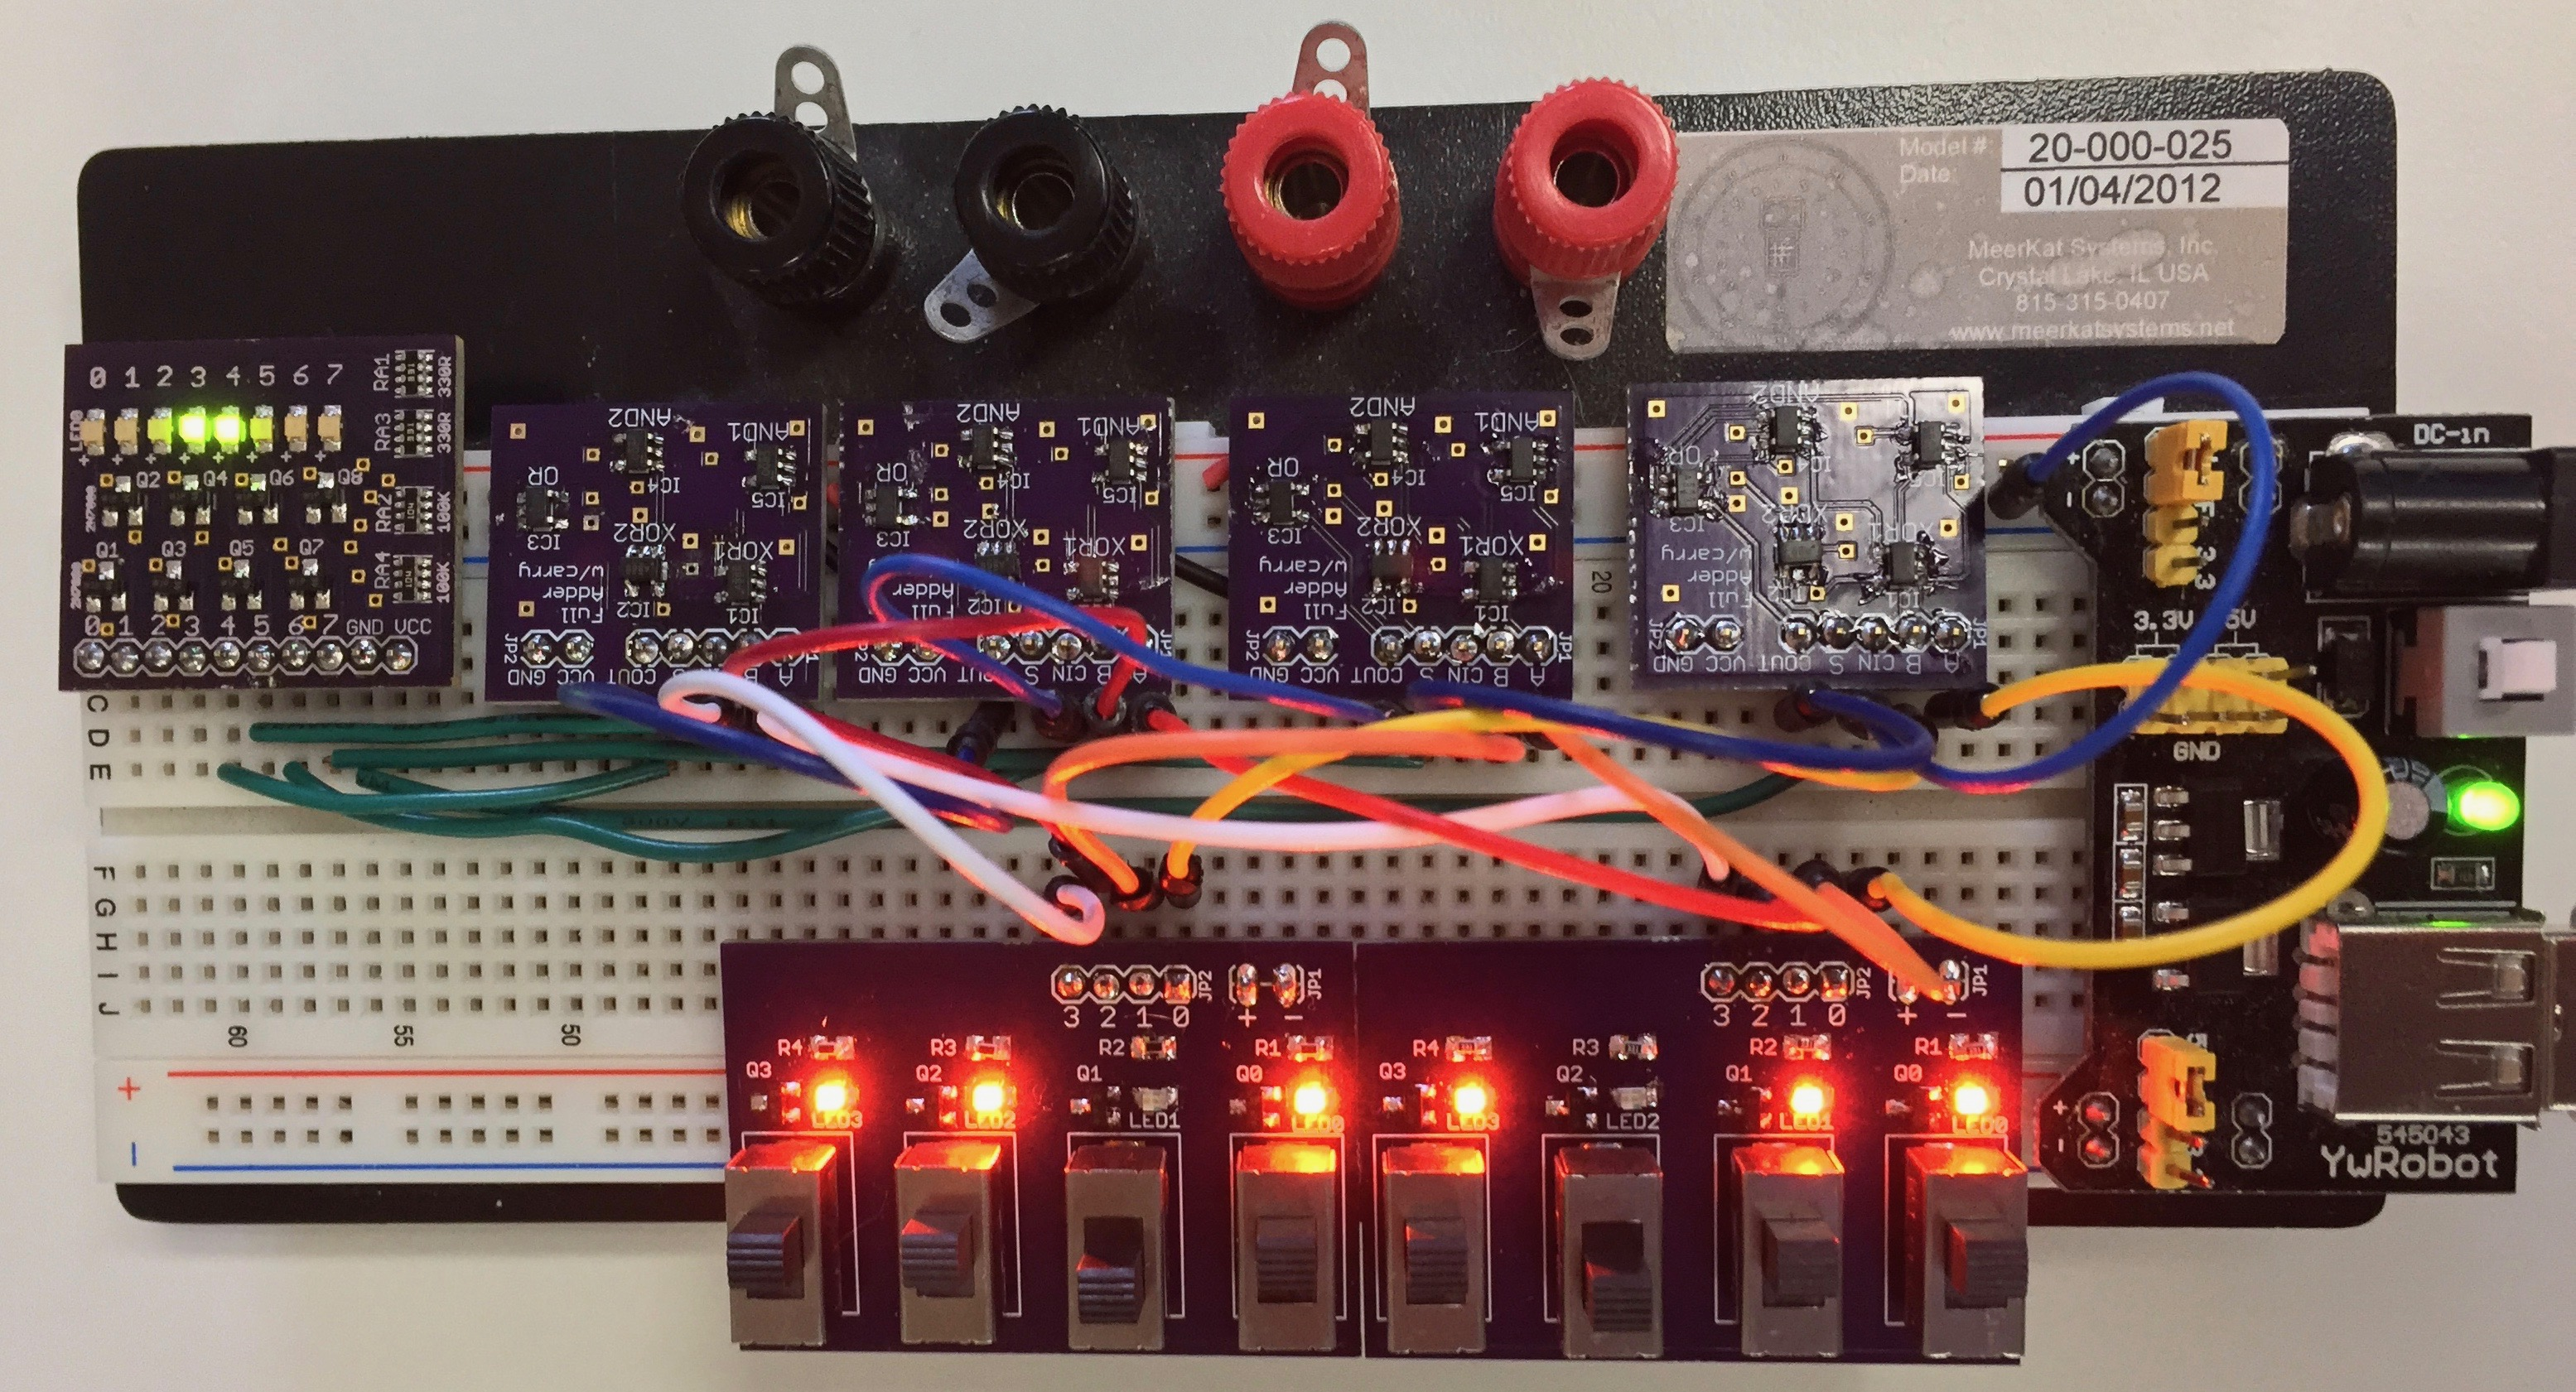
\includegraphics[scale=0.15]{4bitadder.jpg}
\caption{A properly wired 4-bit adder, with a carryout. This setup can count to 30. Here, it is adding ($8 + 4 + 0 + 1$) and ($8 + 0 + 2 + 1$), and the result is 24. The input values are color coded in pairs, so the 1s are yellow, the 2s are orange, the 4s are red, and the 8s are white. The carry-out and carry-in jumpers are blue, and the sum lines (that go to the LEDs) are green.}

\end{figure}

% Subtracting is adding the two's complement (one's complement + 1 );
% so, to subtract, you'll need a vector of NOT gates to get the one's complement,
% plus a trip through the adder circuit for both numbers
% (and someplace to store the result!) before you can implement subtraction.
% Probably only suitable an an appendix to this document because of the 
% additional "moving parts" and the memory requirement (8 latches or SRAM cells isn't
% that much work, but scope creep is already a problem with this project).

